\section{Evaluation and critical appraisal}
\label{s:evaluation}

\hspace{10pt} This section mainly focuses on the analysis of energy efficiency of the components described in this dissertation. In the first subsection, the sensor energy measurements' results are evaluated. Basing on those results, I reach general conclusion and also inspect the sensors used for localization in more details.  In the second subsection, the energy efficiency of Locy is investigated. [XXX go on Locy].

\subsection{Sensor energy measurements}

\hspace{10pt} The Figure \ref{p:all_results} shows the complete set of the experiments results across three different devices. For all of those phones, the time of 1\% battery life depletion is the biggest when all sensors are switched off i.e. "plain" run. Next, all of the physical sensors belongs to the group of less energy-efficient sensors. On the boundary of this group, microphone may be noticed. Finally, IEEE 802.11, GPS and Video Camera have relatively high energy demands on all of the three devices.

\begin{figure}[H]
\centering
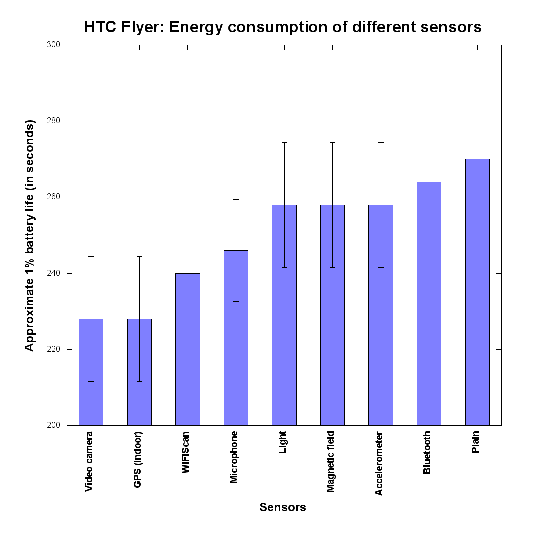
\includegraphics[width=0.49\textwidth, scale=0.6]{plots/htc_flyer}
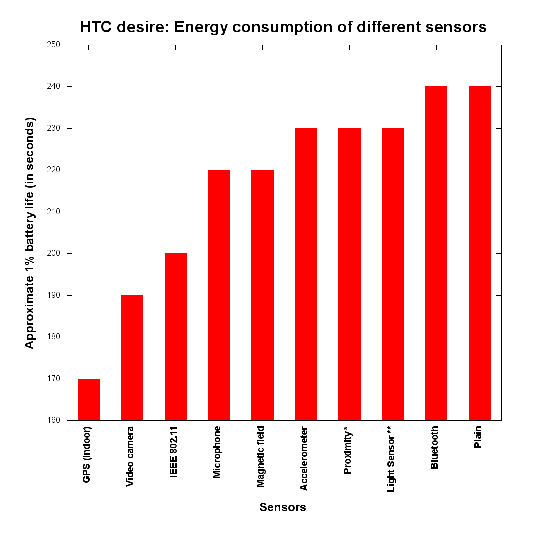
\includegraphics[width=0.49\textwidth, scale=0.6]{plots/htc_desire}
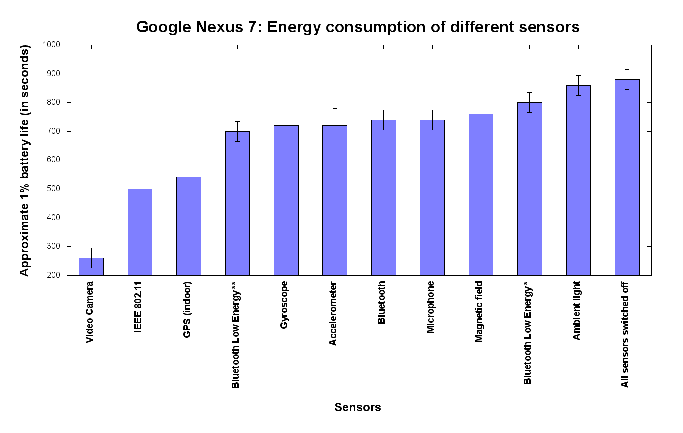
\includegraphics[width=\textwidth, scale=0.9]{plots/google_nexus_7}
\caption{\label{p:all_results} The complete results of energy measurements for all devices. The energy efficiency of different sensors is as expected and overlaps with the results of other research. }
\end{figure}

Bluetooth Low Energy\ (LE) may have higher energy demands than Classic Bluetooth. The \plotref{bluetooth_le_api} compares their energy efficiency depending on the situation. In there is no device found, it takes longer for Bluetooth LE scanning to deplete the battery life by 1\% than for Classic Bluetooth scanning i.e. Bluetooth LE is more energy-efficient. However, if there is any device on the network, Bluetooth LE scanning depletes battery faster than Classic Bluetooth. The reason behind this phenomenon was analyzed in the previous section (the high output of Bluetooth LE API when any device is found) \ref{p:all_results}.
	
\plot{bluetooth_le_api}
				
The energy efficiency order of the sensors differs among the devices. The \plotref{shared} contrasts the energy efficiency results for the shared sensors between the devices.For each of its diagrams, the order of the sensors on x axis is the same. The diagram on the left\ (Google Nexus 7) is characterized by monotonically increasing energy efficiency of the sensors, whereas the other two diagrams are not. For example, Bluetooth is the most energy efficient sensor HTC Desire and HTC Flyer, but is average for Google Nexus 7.

\plot{shared}
		
\subsubsection{Localization}

\hspace{10pt} Different sensors may be used for localization purposes. The \plotref{all_locs} studies the energy efficiency of those sensors. For the comparison, the energy efficiency levels described in the previous section were used. For each of the devices, Bluetooth has the highest energy efficiency level i.e. it is the most energy-efficient. Also, microphone is always more energy efficient than traditional localization sensors\ (GPS and IEEE 802.11). On the other hand, the camera has worse energy performance than GPS and IEEE 802.11 on the two devices. Finally, the energy efficiency of GPS and IEEE 802.11 are similar, though the latter is more energy-efficient for two out of three devices.  	

\plot{all_locs}

Physical sensors are more energy efficient than traditional localization sensors. The energy efficiency of accelerometer is compared with GPS and IEEE 802.11 scanning on the \plotref{acc_vs_loc}. The accelerometer is more energy efficient, but the difference is not always substantial. For HTC Flyer and HTC Desire, the difference between the energy efficiency of accelerometer and traditional localization sensors is less than one energy efficiency level. It is worth reminding here that Accelerometer Sensor Application applies continuous sampling (i.e. sample as often as possible without sleeping intervals).
	
\plot{acc_vs_loc}		

\subsubsection{Conclusions}
\hspace{10pt} The complete set of energy measurements' results are intuitive and overlap with other research, which uses different measurement methods \cite{constandache:localization} \cite{wang:eemss} \cite{chon:smartdc}. This gives validation to the energy measurement method used in this dissertation. For Google Nexus 7, the results confirm the energy-efficiency problems with Bluetooth Low Energy API, which were noticed during the implementation phase. Finally, the energy measurement results vary among different devices. This justifies why the universal power model cannot be used. It also validates the necessity of online energy measurements. 

The analysis of the localization sensors' efficiency explains how localization technologies evolve. Bluetooth, the most energy efficient sensor, is already widely adopted in the industry. iBeacon \cite{apple:ibeacon}, provided by Apple Inc.,  leverages Bluetooth LE for the indoor positioning system. Also, promising energy-efficiency results of microphone attracted research community. SurroundSenses \cite{azizyan:surroundsense} utilizes microphone for localization through ambient sound fingerprinting. Lastly, camera is the most expensive sensor, and thus, computer vision is not yet widely used for localization.

Accelerometer is more energy efficient than traditional localization sensors. Opposite to what previous research\cite{benabdesslem:senseless} stated, the difference in energy consumption is not substantial. The nature of accelerometer usage has been changed. Currently, the values of physical sensors may be pulled more often\ e.g., three accelerometer values are delivered per second on Google Nexus 7. Higher frequency of raw data may have better accuracy, but also results in faster battery depletion.  Because of that, the smarter strategies for sampling needs to be designed. For example, accelerometer may sample for short period of time and if unsure what happens, it could sample longer. As accelerometer has lower energy demands than traditional localization sensors, it could be leveraged for "cheaper" replacement fo those "expensive" sensors. However, its sampling needs to be conducted in energy-efficient manner. 

The energy measurement method does not provide the details on the nature of energy consumption. It is unknown which exact operations consume the most energy during sensing. For example, significant part of energy may be consumed by CPU which needs to be active while sensing accelerometer \cite{priyantha:littlerock}. As those characteristics are not recognized, it cannot be reason how energy efficient the applications with combined sensors\ (IEEE 802.11 scanning and accelerometer) will be. Also, it is unfamiliar how energy efficiency of physical sensors will change depending on their parameters\ (size of sleeping and sampling windows).
						
\subsection{Locy}
-Three different scenarios
-results across three different mobile phones

\plot{locy_eval_inplace}

\plot{locy_eval_other}

\subsection{Conclusions}
The energy measurement method delivered the complete set of accurate energy efficiency results, and thus, the method was validated. The results were gathered across three different mobile phones and include all sensors. It is believed that it is first study of this type. 

Physical sensors could be leveraged for localization purposes. The energy efficiency results gave a basis for how an energy-efficient library could be designed. The energy measurement method provided useful information and identified the challenges for Locy. The energy efficiency of combined sensors and different energy efficiency of physical sensors depending on their parameters needed to be checked. 

Those challenges were met by Sensy. XXX...